\documentclass[12pt, letterpaper]{article}
\usepackage[utf8]{inputenc}
\usepackage{amsmath}
\usepackage{parskip}

\usepackage{graphicx}
% \usepackage[]{svg}

\graphicspath{{../images/}}

\usepackage{hyperref}
\hypersetup{
    colorlinks=true,
    urlcolor=blue,
    linkcolor=blue,
    citecolor=blue,
    filecolor=blue,
}
\urlstyle{same}

\title{Notes to Fully Connected Neural Network}
\author{}
\date{}


\begin{document}

\maketitle
\tableofcontents
\setcounter{tocdepth}{3}

\section{Architecture}

When the main Neural Network enters the data pipeline, all input variables have already been transformed to numeric predictors, i.e. originally categorical variables are encoded as \textit{Dummy} Vectors and inherently numeric variables are zero centered and scaled to unit variance.
Thus, both the price variable as the outcome as well as all predictor variables can be transformed to \textbf{Tensors}, the canonical data type across all popular Deep Learning Frameworks.

The network design choice was only restricted by two factors:
%%%
\begin{enumerate}
    \item The number of input features in the \emph{first} layer necessarily equals the number of features contained in the input data set.
    \item The number of output features in the \emph{last} layer is fixed to $1$, since the network directly predicts the price as a single scalar.
\end{enumerate}
%%%
Hence, both the \emph{width} and the \emph{depth} of the network as well as all intermediate components are free to choose.

After experimenting with many different configurations that proved to empricially be beneficial in the literature, we finally settled with a fairly simple \emph{block structure}.

Starting from roughly $60$ input features, the network width is first blown up to $256$ features and then, almost symmetrically, steadily decreased to the single output neuron in the final layer.
More precisely, the architecture consists of $6$ \textbf{blocks} with $64$, $128$, $256$, $128$, $64$ and $8$ output features in addition to the first linear layer connecting the input features with the first block and the last layer connecting the last block with the prediction output.

%%%
\begin{figure}[ht]
    \centering
    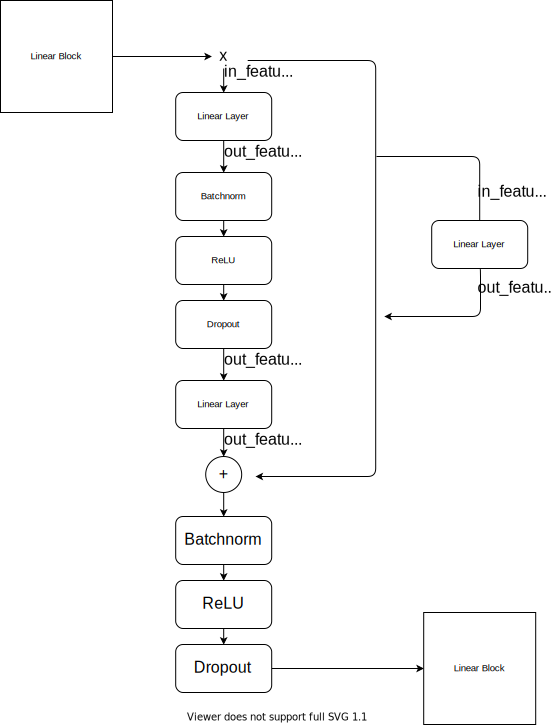
\includegraphics[width=\textwidth]{mlp_architecture.png}
    \caption{Architecture of each Block in the Fully Connected Neural Network}
    \label{fig:linear-block}
\end{figure}
%%%

The structure of each so-called \texttt{Linear Block} is displayed in figure \ref{fig:linear-block}.
The following paragraph explains the reasoning behind including or excluding elements in this configuration.

\textbf{Linear Layer} \\
Each \texttt{Linear Block} is based on a four-element cycle that is repeated twice.
Each cycle starts with a Fully-Connected Layer containing the majority of trainable weights in the network.
The first linear layer determines the output dimension of the block, in our case mostly doubling or halving the number of input features for this block.
Since both linear layers are immediately followed by a \texttt{Batchnorm} Layer, the additional \texttt{Bias} term is redundant (vanishes due to centering during Batchnorm) and is therefore omitted.

\textbf{Batchnorm} \\
\texttt{Batchnorm} Layers are often connected to a more well-behaved training process.
By means of first standardizing teh activations within each minibatch and rescaling them afterwards, the networks \emph{learns} a convenient magnitude of the activations.
This tends to be particularly impactful for \emph{saturating} activating functions such as the \texttt{sigmoid} or \texttt{tanh} activations, however positive effects for training have also been observed for the \texttt{ReLU} activation function, which is used in our design.
Of all individual components of the \texttt{Linear Block} structure, Batchnorm was the least important and only provided marginal benefits.

\textbf{ReLU} \\
Out of the numerous options for including nonlinearities into the network and thus expanding the function space that the network is able to learn, we settled for the default choice of the \emph{Rectified Linear Unit} activation.
While briefly experimenting with its cousins, the \texttt{Leaky ReLU} and the \texttt{Exponential ReLU} the differences were barely noticeable and could be just as well attributed to other factors such as the random weight initialization.

\textbf{Dropout} \\
The \texttt{Dropout} Layer at the end of each cycle turned out to be the single most impactful factor for \emph{generalization} ability.
In fact, due to the different behaviour of dropout during training and inference, we could directly control the relative performance on training and validation set by varying the dropout probability $p$.
By setting $p$ to zero the network overfitted drastically.
This was actually a very important observation proving that the current function class is flexible enough to model the task at hand properly.
Thus, there was no need to artificially expand the network size further, which kept the architecture quite compact with roughly $280.000$ trainable parameters and saved a lot of computation time.

%%%
\begin{figure}[ht]
    \centering
    \includegraphics[width=\textwidth]{dropout_performance.png}
    \caption{Impact of Dropout Probability on Training and Validation Performance}
    \label{fig:dropout}
\end{figure}
%%%

Figure \ref{fig:dropout} displays the shift in performance metrics on training and validation set when steadily increasing the dropout probability $p$.
While not beneficial for overall performance, the dropout delivers a leverage to let the model perform much better on out of sample data compared to the dataset that it actually trained on.
This behaviour can be explained by the \emph{ensemble} interpretation of dropout:
In each epoch, a different subset of neurons is excluded to contribute to training and thus a distinct subset model nested in the full model is responsible for the prediction output.
If the dropout probability is extremely high, these subset models are simply too different from each other and \emph{do not agree} on a common range of sensible prediction values.
In contrast, during inference (and possible deployment of the model), any randomness should be avoided and the network may use all of its neurons.
Although there is no influence on the model \emph{weights} in this stage, the model pools all small subset models together and \emph{averages out} the diverging effects of each component resulting in better performance metrics.

\textbf{Residual Connections} \\
One special feature of the \texttt{Linear Block} architecture is the \emph{Residual Connection} adding the block input to the output of the second linear layer within each block.
This component was originally implemented with the thought of a fairly deep network in mind since \emph{Residual Blocks} introduced by the famous \texttt{ResNet} architecture are arguably the most popular tool for a stable gradient flow by preventing the issue of vanishing gradients.
As mentioned above the depth of the final model turned out to be limited.
We decided to enable inclusion and exclusion of skip-connections in the network by a simple \texttt{boolean} input to the main model fitting function allowing for easy comparisons between the model designs.
Although the residual component did not have a major impact on performance, it was slightly beneficial in most settings such that there was no reason to remove it from the model.


\section{Hyperparameters and Further Remarks}

This subsection discusses why we chose to leave out certain elements from the model architecture and stated the default values for all other hyperparameters contributing to the network.

% TODO: learning rate/learning rate schedulers, batch size, weight decay



\section{Influence of the price distribution}

% TODO: extremely sensitive to outliers, log price did not help => training more difficult, futher investigation and explanations with VAE => include plot of latent space representation, dataset not expressive enough to capture all factors contributing to very high prices, general discussion about validity of data


\newpage

\bibliography{bib}
\bibliographystyle{apalike}

\end{document}